\chapter{Cell Differentiation }\label{celldiff}
\lhead[\fancyplain{}{\bfseries\thepage}]{\fancyplain{}{\bfseries\rightmark}}

In this Chapter we explain Cell Differention process and Gene Regulatory Networks.

\section{Definition}
Cell differentiation is the process whereby stem cells become progressively
more specialized. The differentiation process occurs both during the devel-
opment of a multicellular organism and during tissue repair and cell turnover
in the adulthood. Gene expression, and therefore its regulatory mechanisms,
plays a critical role in cell differentiation.
\begin{figure}
\centering
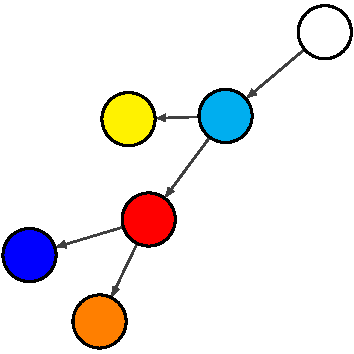
\includegraphics[angle=45]{images/cells.pdf}
\caption{\emph{Schematic representation of cellular differentiation.}}
\end{figure}
Stem cells are undifferentiated biological cells which can both reproduce
themselves, self-renewal ability, and differentiate into specialized cells, potency.
The principles underlying cellular differentiation remain among the most
enigmatic in biology. We are required to explain the spontaneous generation of a multiplicity of cell types from the single zygote, to deduce a natural
tendency of a system to become increasingly heterogeneous, then to stop
differentiating.

Among the important characteristics of cell differentiation are: 
\begin{itemize}
\item initiation
of change; 
\item stabilization of change after cessation of stimulus; 
\item the efficacy of
many substances, exogenous and endogenous, as inductive stimuli;
\item progressive limitation in the number of developmental pathways open to any small region of the embryo; 
\item restricted periods during which
a cell is competent to respond to an inductive stimulus; the discreteness of
cell types, that is, the mutually exclusive constellations of properties by
which cells differ; 
\item a requirement for a minimal and preferably heterogeneous
cell mass to initiate differentiation in many instances, and to maintain it in
some; 
\item the occurrence of metaplasia between undifferentiated cell types, or
from an undifferentiated type to a specialized type, but the lack of metaplasia
(the isolation) between specialized cell types; 
\item cessation of differentiation.
\end{itemize}

Cells are thought to differ due to differential expression of, rather than
structural loss of, the genes. Differential activity of the genes raises at least
two questions which are not always carefully distinguished: the capacity of
the genome to behave in more than one mode; and mechanisms which insure
the appropriate assignment of these modes to the proper cells.



Within multicellular organisms, tissues are organized in communities of cells that work together to carry out a specific function. The exact role of a tissue in an organism depends on what types of cells it contains. For example, the endothelial tissue that lines the human gastrointestinal tract consists of several cell types. Some of these cells absorb nutrients from the digestive contents, whereas others secrete a lubricating mucus that helps the contents travel smoothly.
However, the multiple cell types within a tissue don't just have different functions. They also have different transcriptional programs and may well divide at different rates. Proper regulation of these rates is essential to tissue maintenance and repair. 
Stem cells typically have the capacity to mature into many different cell types. \emph{Transcription factors} (TF), which are proteins that regulate which genes are transcribed in a cell, appear to be essential to determining the pathway particular stem cells take as they differentiate. For example, both intestinal absorptive cells and goblet cells arise from the same stem cell population, but divergent transcriptional programs cause them to mature into dramatically different cells.
Whenever stem cells are called upon to generate a particular type of cell, they undergo an asymmetric cell division. With asymmetric division, each of the two resulting daughter cells has its own unique life course. In this case, one of the daughter cells has a finite capacity for cell division and begins to differentiate, whereas the other daughter cell remains a stem cell with unlimited proliferative ability.

\section{The role of Gene expression in cellular differentiation}
Gene expression is a complex process regulated at several stages in the synthesis of proteins. In addition to the DNA transcription regulation, the expression of a gene may be controlled during RNA processing and transport (in eukaryotes), RNA translation, and the post-translational modification of proteins. This gives rise to genetic regulatory systems structured by networks of regulatory interactions between DNA, RNA, proteins and other molecules: a complex network termed as a \emph{gene regulatory
network} (GRN). Some kind of proteins are the transcription factors that bind to specific DNA sequences in order to regulate the
expression of a given gene. The power of transcription factors resides in their ability to activate and/or repress transcription of genes. The activation of
a gene is also referred to positive regulation, while the negative regulation
identifies the inhibition of the gene.
The regulation of gene expression is essential for the cell, because it
allows to control the internal and external functions of the cell. Furthermore,
in multicellular organisms, gene regulation drives the processes of cellular
differentiation and morphogenesis, leading to the creation of different cell
types that possess different gene expression profiles, and these last therefore
produce different proteins that have different ultrastructures that suit them
to their functions. Therefore, with few exceptions, all cells in an
organism contain the same genetic material, and hence the same genome. The difference between the cells are emergent and due to regulatory mechanisms which can turn on or off genes. Two cells are different, if they have different subsets of active genes.
